
%https://wstein.org/edu/2007/spring/ent/ent-html/node89.html
\Section{Elliptic-curve cryptography \& ECDSA}\label{ecdsa}
As covered in the introduction, Elliptic-curve cryptography (\textbf{ECC}) and ECDS (Elliptic curve digital signature) 
is a fundamental building block of bitcoin. Elliptic curve cryptography relies on 
intractability of calculating the discrete logarithm of a elliptic curve element with 
respect to a publicly known base point.\cite{miller_1986}\cite{nakamoto_bitcoin}\cite{antonopoulos_2017}\cite{ecc_def} Or put another way: It is easy to calculate 
elliptic curve multiplication with multiplicand $n$. But calculating $n$ from the 
resulting point is considered infeasible with sufficiently large curves and multiplicands.\cite{antonopoulos_2017}

%Not sure about the field
An elliptic curve is defined by the equation $Y^2=x^3+ax+b$ and six domain parameters 
$E(p,a,b,G,n,h)$.\cite{Secp256k1_def}\cite{ecc_def} $\textbf{p}$ is the field that the curve is defined over, this 
is usually a very large prime number. The curve being defined over a field simply 
means that the points on the curve fall within $[0, p]$ rather than within the 
real numbers $\mathbb{R}$. In other words the curve is defined over the field 
$\mathbb{F}_{p}$. $\textbf{a}$ and $\textbf{b}$ are whatever number you put into 
the equation. $\textbf{G}$ is the generator point, that is the point on the curve 
that will be used in point multiplication later. $\textbf{n}$ is the order of G. What 
that means is that $n$ is the largest number that $G$ can be multiplied by before 
a point at infinity is produced. $n$ pretty much tells you the limit on how many points 
on the curve that can be generated from $G$. $\textbf{h}$ is the co-factor of the 
curve. It can be calculated as follows: $h=\frac{1}{n}|(E(\mathbb{F}_{p})|$, where 
$|(E(\mathbb{F}_{p})|$ is the order/cardinality of the group of points possible on 
the curve over field $\mathbb{F}_{p}$. $n$ is derived from $G$, $G$ and $p$ should 
be chosen in such a way that $h \leq 4$, preferably $h=1$.

These domain parameters can be chosen manually or you can use predefined parameters. 
Elliptic curves that used predefined domain parameters are called named-curves. 
The named curve used by Bitcoin is called \texttt{Secp256k1}.\cite{Secp256k1_def}\cite{antonopoulos_2017}\cite{nakamoto_bitcoin}

\Subsection{Secp256k1}
\texttt{Secp256k1} is defined with the following domain parameters (hexadecimal):\\\\
$p=\texttt{FFFFFFFF FFFFFFFF FFFFFFFF FFFFFFFF FFFFFFFF FFFFFFFF FFFFFFFE FFFFFC2F}$\\
or alternatively:\\
$p=2^{256}-2^{32}-2^{9}-2^{8}-2^{7}-2^{6}-2^{4}-1$

$a=0$\\
$b=7$

$G=(\texttt{79BE667E F9DCBBAC 55A06295 CE870B07 029BFCDB 2DCE28D9 59F2815B 16F81798},\\ \null\qquad\:\:\: 
\texttt{483ADA77 26A3C465 5DA4FBFC 0E1108A8 FD17B448 A6855419 9C47D08F FB10D4B8})$


$n=\texttt{FFFFFFFF FFFFFFFF FFFFFFFF FFFFFFFE BAAEDCE6 AF48A03B BFD25E8C D0364141}$
$h=\texttt{1}$

\Subsection{Math on the elliptic curve}
Two mathematical operations needs to be defined to operate on the elliptic curve: 
addition and multiplication, as they are defined by \textbf{SECG} (Standards For Efficient CryptoGraphy). In their paper: SEC 1: Elliptic curve cryptography.\cite{ecc_def}

\Subsubsection{Point addition}
Let's say you have to distinct points P and Q that both fall on curve $E(p,a,b,G,n,h)$ 
($Y^2=x^3+ax+b$). 

$$P+Q=R \Rightarrow (X_P, Y_P) + (X_Q, Y_Q) = (X_R, Y_R)$$

$$X_R = \lambda^2-X_P-X_Q$$
$$Y_R = \lambda(x_P-X_R) -Y_P$$

where $\lambda$:

$$\lambda = \frac{Y_Q-Y_P}{X_Q - X_P} \mod p$$

\Subsubsection{Point multiplication}
If P and Q are coincident, meaning that they have the same coordinates the equation 
is slightly different. 

$$P+Q=R \Rightarrow P+P=R \Rightarrow 2P=R$$ 

This could be seen as P being multiplied with scalar 2. Most of the equation is the same 
as with addition, the difference is that:\\
$$\lambda = \frac{(3X^2_P + a)}{(2Y_P)} \mod p$$

\Subsubsection{Faster multiplication with large scalars}
Take $xP=R$ that could be calculated by summing P x times:
$$\sum_{n=1}^{x} P = R$$
This might work fine for smaller numbers but for a very large number, like $x=2^{100}$, it will 
take infeasible amount of time to calculate. Luckily there is a convenient short cut that you 
can take called double and add. 

First remember that: $P+P = 2P \Rightarrow 2P + P = 3P \Rightarrow 4P = 2(2P) \Rightarrow 8P = 2(2(2P))$

Lets say $x=200$ in binary terms this could be written as $x=128+64+8$ or $x=2^7+2^6+2^3$ 
thus $200P=R$ could be written as 
$$2^7P+2^6P+2^3P=R$$ 
which can be expanded to: 
$$2(2(2(2(2(2(2P)))))) + 2(2(2(2(2(2P))))) + 2(2(2P))$$ 
This looks more cumbersome but now instead of 200 calculations you only have to do 19, or more exactly instead of 200 elliptic-curve additions you have to do 3 elliptic-curve additions and 16 elliptic-curve multiplications


\Subsection{Private and public key}
Just as \texttt{RSA} cryptography, ECC relies on public-private key encryption and signatures. 
The public key can be shared freely to everyone, while the private key should, as the name implies, 
be kept private. Each unique private key has a corresponding public key, through mathematics it 
can be proven that someone holds the private key paired with a certain public key, without actually 
revealing the private key.\cite{antonopoulos_2017}\cite{Secp256k1_def}

\begin{wrapfigure}{r}{0.3\textwidth}
	\begin{center}
		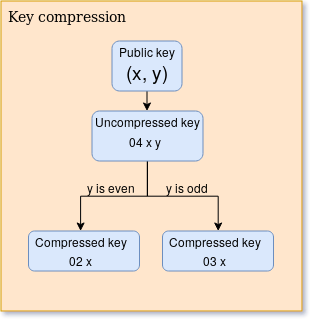
\includegraphics[width=0.4\textwidth]{background/images/key_compression.png}
	\end{center}
	\vspace{-8mm}
	\caption{How to compress the public key in ecc}
\end{wrapfigure}

In ECC \textbf{a private key is a really large number}. Imagine you have curve $E(p,a,b,G,n,h)$ 
and you want to generate a brand new private key k. k could be any number between 0 and $n$. Any 
$k > n$ will produce the exact same public key so that will not work. \textbf{A public key in ECC is 
represented by a point in 2D space}, more specifically a point that falls on the curve.\cite{antonopoulos_2017} To generate a 
public key P from a private key k you perform $kG = P$ as described in the section above.\cite{ecc_def}\cite{Secp256k1_def}

\Subsubsection{Compressed key}
The public key is quite large, with two 256-bit numbers representing coordinates. But there is a 
clever trick we can use to compress the size of the key. Take the \texttt{Secp256k1} curve for 
example ($Y^2=x^3+7$). It is mirrored around the x-axis, meaning that for each x value there 
are two possible y values. Thus a public key can be represented by only it's x value plus a 
prefix telling you which resulting y-value to choose.\cite{antonopoulos_2017}

Note that because y and x is over $\mathbb{F}_{p}$ there is no negative value, instead the y 
value is referred to as even or odd. 




\Subsection{ECDSA}
The main usage of ECC in cryptocurrency is for proving ownership of coins.\cite{antonopoulos_2017}\cite{nakamoto_bitcoin} The proof relies 
on elliptic curve mathematics like before. Lets say \textbf{Alice} has a message $m$ and want 
to send it to \textbf{Bob} and also prove that the message came from her. First of let's 
establish some variables: $k_A$ is the private key belonging to Alice, and from it the public key $P_A$ was generated. Bob knows $P_A$ but not $k_A$ 

The signature generation and validation are as described by \textbf{SECG} (Standards For Efficient CryptoGraphy). In their paper: SEC 1: Elliptic curve cryptography.\cite{ecc_def}

\Subsubsection{Signing}
First calculate the hash of the message:
$$e=HASH(m)$$
If $e$ has a bit-length (numbers in binary representation) that is longer than the bit-length 
of order $n$ of the curve used. $e$ has to be trimmed down so that the bit-lenghts match

Select a cryptographically-secure random number $z$ that falls in the range $[1, n-1]$ and 
calculate a new curve point: $(x_1, y_1) = z \times G$

Calculate $r$ and $s$ such that: $r = (x_1 \mod n)$ and $s = (z^{-1} (e + r \times k_A) \mod n)$. 
if either $r$ or $s$ ends up being 0, generate a new $z$ and try again.

The signature will be the point $(r, s) = S_A$.

\Subsubsection{Signature validation}\label{signature_validation}
If \textbf{Bob} wants to verify that it was actually \textbf{Alice} that signed the message $m$. 
He first has to do a sanity check on the signature $S_A$ to make sure that it is a valid point on 
the curve and that $s$ and $r$ is within the range $[1, n-1]$ etc... 

Calculate the hash $e$ of $m$ the same way as it was done during the signing process. Calculate 
$$w=(s^{-1} \mod n)$$ and $$u_1 = (ew \mod n)$$ $$u_2 = (rw \mod n)$$

From $u_1$ and $u_2$ calculate the point $(x_1, y_1) = u_1 \times G + u_2 \times S_A$ 

The signature is valid if and only if $r = x_1 \mod n$

\Subsection{Addresses}
While using Bitcoin normally you rarely interact with the public keys directly, instead you mostly see  and use something that is called addresses.\cite{antonopoulos_2017} For example if you want to send money to someone you use their bitcoin-address (see section \ref{p2pkh}). What the address really is, is just a obfuscated representation of a public key.  

To transform a public key to an address you first hash it using \texttt{SHA256} then hash the result of that with \texttt{RIPEMD160}, this entire process is called HASH160. After doing HASH160 you encode the resulting bytes in Base58, this is your address.\cite{antonopoulos_2017}

HASH160($P_A$) = RIPEMD160(SHA256($P_A$))\\
$A_A$ = BASE58(HASH160($P_A$))

For example:

Compressed public key:\\
\texttt{03b2319bf63ca8959794f79056283150f1b49d577b2c48bd9e4a18d616e6f99bb4}

Hash160 of public key:\\
\texttt{76a9147ecfe7db089f521c3f49de0ee866f8e0fee97d1788ac}

Base58 of public key hash (Address):\\
\texttt{ms5UVmKaaz8kiL7DbMA1NG3t6T4C4GmGzG}

\Subsection{Homomorphism}\label{homomorphism}
Elliptic curves has a attribute called homomorphism. It will not be covered in depth, but what it can be used for is that two public keys ($P_1$, $P_2$) can be combined to form a third public key ($P_R$). If $P_1$ and $P_2$ was generated with corresponding private keys $k_1$ and $k_2$ then they can be combined to form the private key that generates $P_R$ ($k_R$).\cite{miller_1986}\cite{bolt}

There are several ways of calculating a new homomorphic key, this is the one used in later implementations:

Let's say you have private key k with corresponding public key P. And another temporary private key $k_c$ with corresponding public key $P_c$. To generate the homomorphic public key ($P_h$) you can use the following equation (All the operations in equation \ref{generate} below are in elliptic-curve addition and multiplication. The second (\ref{resolve}) uses regular operators):

\begin{equation}\label{generate}
Generate(P, P_c) = P * SHA_{256}(P || P_c) + P_c * SHA_{256}(P_c || P) = P_h
\end{equation}

You now have Public key $P_h$. To figure out the Private key correlated with this public key you do the following equation:

\begin{equation}\label{resolve}
Resolve(k, k_c) = k * SHA_{256}(P || P_c) + k_c * SHA_{256}(P_c || P) = k_h
\end{equation}

\Subsubsection{Revocation keys}
Imagine Alice and Bob wanting a public key that neither hold the private key to, that could be revealed at a later date. Alice holds the key set ($k_A$, $P_A$), and Bob has the set ($k_B$, $P_B$). Bob creates another key set ($k_T$, $P_T$) and sends $P_T$ to Alice.

Alice generates a new public key ($P_R$) from $P_A$ and $P_T$ with equation \ref{generate}. Now the public key $P_R$ could be used for whatever purpose needed, even though neither party knows the private key $k_c$ at this point as calculating it requires both $k_A$ and $k_T$ and neither party holds both. At a later date Bob could reveal $k_T$ to Alice, she could then use equation \ref{resolve} to determine $k_R$.\cite{bolt}

This method is used later in a concept called revocable deliveries, see section \ref{breach_remedy}. In that case ($k_T$, $P_T$) key set would be called commitment point keys, and ($k_R$, $P_R$) would be called revocation keys.\cite{bolt}